\section{Demonstração Prática}
De modo a exemplificar os conceitos enunciados no capítulo II, foi realizada uma demonstração prática que almejou, fundamentalmente, constituir uma BOTNET de pequena dimensão, num ambiente controla. Assim, foram desenvolvidas diversas ferramentas, com o apoio de bibliotecas \textit{open source},que possibilitaram o estabelecimento de um fluxo automático de informação entre um operador humano e um alvo digital.

Neste seguimento, o ambiente em questão, foi implementado localmente, mediante utilização de uma rede local, assim como 3 computadores. Mais se acrescenta que, 2 dos computadores desempenharam o papel de \textit{bot}, enquanto que o restante dispositivo desempenhou o papel de servidor C2 e sistema alvo.

\subsection{Processo de \textit{Setup}}
Para a implementação do ambiente, foi utilizada a linguagem de programação Python, mais especificamente a versão 3.12 desta mesma, já que as versões posteriores apresentam diversos problemas de compabilidade com as bibliotecas empregues.


Deste modo, cumpre esclarecer as ferramentas utilizadas pelos intervenientes da demonstração prática, a saber:
\begin{itemize}
    \item \textit{Bots}: funcionalidades de DoS disponibilizadas pelo projeto Bane \cite{github_bane}. Nesta senda, cabe notar que foram utilizados o módulo relacionado com um ataque DDoS. De modo a instalar este, foi necessário utilizar a supramencionada versão do Python, assim como efetuar a importação deste. Mais se acrescenta que os \textit{bots} possuem um servidor cliente próprio, cujo possiblita a comunicação com o controlador C2 e, consequentemente, a obtenção de comandos e o envio de relatórios para este, procurando clarificar o estado das operações.
    \item Servidor C2: qualquer servidor capaz de receber pedidos HTTP será suficiente. Assim, foi empregue a ferramenta Flask, que se revelou curial às necessidades da demonstração.
    \item Servidor Alvo: foi constituido um servidor simples que somente regista os pedidos que recebe. Mais se acrescenta que foi utilizado o módulo Beszel \cite{github_beszel}, de modo a monitorizar o tráfego recebido, já que este possuí requisitos mínimos de implementação.
    \item Operator: procura comunicar com o servidor C2, via pedidos HTTP. De modo a possibilitar isto mesmo, foi disponibilizada, em formato de texto, a totalidade de comandos \textit{Invoke-WebRequest} possíveis no ficheiro "c2\_server\_commands".
\end{itemize}

\subsection{Arquitetura e Execução}
No âmbito da arquitetura de sistema implementa, cabe notar que esta se encontra dividida em 4 setores, a saber: operador; servidor C2; \textit{bots}; servidor alvo. Neste seguimento, a Figura \ref{fig:arquitetura-testes} apresenta o fluxo de informação desta mesma arquitetura.


\begin{figure}[!h]
    \centering
    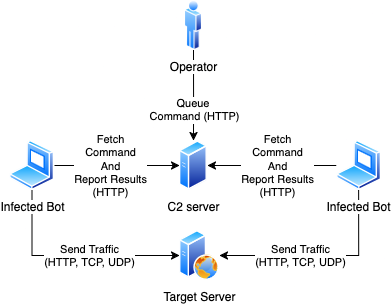
\includegraphics[width=2.5in]{imgs/architecture_smaller.png}
    \caption{Arquitetura do ambiente de teste}
    \label{fig:arquitetura-testes}
\end{figure}


Assim, é possível observar que o processo inicia no operador, que envia um pedido HTTP ao servidor C2. Este pedido contém a instrução sobre o tipo de ataque a ser executado pelos \textit{bots}. Neste seguimento, importa realçar que o servidor C2 encontra-se preparado para escutar pedidos provenientes do operador, mas também dos \textit{bots}. Assim, aquando da receção de um pedido, o servidor C2 armazena este numa fila até ao seu processamento ou coleta pelo mecanismo \textit{garbage collector}. Mais se acrescenta que as instruções de ataque somente podem ser interpretadas pelos \textit{bots} 1 vez, garantindo a unicidade da execução.

Nesta senda, paralelamente ao processo suprarreferido, os \textit{bots} efetuam requisições ao servidor C2 de forma cíclica, verificando, inclusivamente, a existência de novos ataques na fila. Assim, quando um pedido é identificado, o servidor proporciona as instruções necessárias para que cada \textit{bot} compile os resultados do \textit{stdout} e do \textit{stderr} do procedimento de ataque, limitando esta captura aos últimos 300 caracteres. Este limite, via uma análise efetuada, demonstrou ser suficiente para determinar a correta execução do ataque, assim como obter informações relevantes sobre o processo.


Posteriormente, o \textit{bot} retorna ao estado de monitorização, verificando se há novos comandos disponíveis na fila, repetindo-se assim o ciclo. Cumpre, ainda, salientar que os \textit{bots} possuem a capacidade de executar 5 tipos distintos de ataques, conforme as instruções recebidas do servidor C2, a saber: HTTP\_PUNCH; HTTP\_SPAM; TCP\_FLOOD; UDP\_FLOOD e SLOW\_READ. Mais se acrescenta que estes ataque permitem assegurar a diversidade e a flexibilidade nas estratégias ofensivas.


\subsection{Resultados obtidos}
Após a conclusão da constituição do ambiente, foram realizadas diversas rondas de testes para cada um dos ataques supramencionados, cujos dados podem ser consultados nas nas Tabelas \ref{tab:table-idle}, \ref{tab:table-1-bot} e \ref{tab:table-2-bots}. Neste seguimento, cabe notar que todos os ataques foram realizadas via servidor C2, possuíndo uma duração máxima de 30 segundos. Mais se acrescenta que os computadores empregues estavam equipados com o sistema operativo Windows 11 e somente possuíam a aplicação de linha de comandos em execução durante os testes.


\renewcommand{\tablename}{Tabela}
\begin{table}[!h]
    \renewcommand{\arraystretch}{1.3}
    \caption{Análise de métricas em estado \textit{idle}}
    \label{tab:table-idle}
    \centering
    \begin{tabular}{|c|c|}
        \hline
            & \textit{Idle} \\
        \hline
        NET & 7Kb           \\
        \hline
        CPU & 1.5\%         \\
        \hline
    \end{tabular}
\end{table}


\begin{table}[!h]
    \renewcommand{\arraystretch}{1.3}
    \caption{Análise de métricas com a utilização de 1 \textit{bot}}
    \label{tab:table-1-bot}
    \centering
    \begin{tabular}{|c|c|c|c|c|c|}
        \hline
            & H\_P & H\_S  & T\_F  & U\_F  & S\_R \\
        \hline
        NET & 6MB  & 7MB   & 1.3MB & 170Kb & 20Kb \\
        \hline
        CPU & 4\%  & 7.5\% & 6\%   & 8\%   & 3\%  \\
        \hline
    \end{tabular}
\end{table}

\begin{table}[!h]
    \renewcommand{\arraystretch}{1.3}
    \caption{Análise de métricas com a utilização de 2 \textit{bots}}
    \label{tab:table-2-bots}
    \centering
    \begin{tabular}{|c|c|c|c|c|c|}
        \hline
            & H\_P & H\_S & T\_F & U\_F  & S\_R \\
        \hline
        NET & 8MB  & 9MB  & 2MB  & 200Kb & 30Kb \\
        \hline
        CPU & 5\%  & 8\%  & 7\%  & 13\%  & 3\%  \\
        \hline
    \end{tabular}
\end{table}

Mediante análise às informações suprarreferidas, é possível compreender que estas proporcionam uma perspetiva abrangente das condições experimentais do ambiente, assim como dos resultados obtidos. Deste modo, é possível tirar ilações sobre a potencial magnitude de um atacante utilizando uma BOTNET, mais especificamente quanto maior a cifra de dispositivo maior será o impacto do ataque. Mais se acrescenta que, embora não tenham ocorrido repercurssões significativas, o sistema de testes, ao ser submetido a uma BOTNET mais populadada seria capaz de ser derrubado.